%!TEX TS-program = xelatex
%!TEX root = ../../maxwell2018thesis.tex

\chapter[Information Retrieval]{Information Retrieval:\\A History and Background}\label{chap:ir_background}
Search today is ubiquitous, and is now commonplace due to the proliferation of the~\gls{acr:www} and commercial search engines\footnote{Or, as we refer to them in this thesis, \emph{retrieval systems.}} such as \emph{Google} and \emph{Bing}. Despite potential negatives that these technologies may bring -- turning us into \emph{shallow thinkers}~\citep{carr2008google_stupid}, for example -- retrieval systems today by and large make our lives easier, allowing us to find the proverbial needle in the haystack with minimal effort. This is achieved while often attaining near perfect accuracy~\citep{vaughan2004new_measurements}.

\begin{figure}[h]
    \centering
    \vspace{4mm}
    \resizebox{1\hsize}{!}{
    
\includegraphics{figures/ch2-searchbox.pdf}}
    \label{fig:searchbox}
    \vspace{-5mm}
\end{figure}

The field of~\glsfirst{acr:ir} has been long established, and has led to the development of the associated technologies that make the contemporary retrieval systems that we use possible. One of the key developments was the creation of a \emph{de facto} approach to studying~\gls{acr:ir}, along with the various \emph{retrieval models} and means with which to evaluate their effectiveness. This chapter provides an overview of the history of~\gls{acr:ir}, before we move on to discussing the basics of what constitutes an~\gls{acr:ir} system. From there, we discuss the basics of~\gls{acr:iir} before moving onto how evaluation has evolved in the field, moving over a spectrum from the \emph{system} to the \emph{searcher.} Included in our discussion of the searcher are some of the current searcher models with which we improve upon, before we conclude the chapter with a discussion of the various measures used for evaluation of both system and searcher.

\section{A (Brief) History of Information Retrieval}\label{sec:ir_background:history}
While many associate the study of~\gls{acr:ir} with computers, the need to seek information in a quick and effective manner has existed throughout human history. In this section, we provide a very brief overview of some of the key advancements in what can be considered to be the study of~\gls{acr:ir} -- from library cataloguing approaches to contemporary retrieval systems.

 %This ranges from library indexing systems, to more contemporary retrieval systems that deal with the enormous volumes of content available on the~\gls{acr:www}.

\subsection{Libraries and Mechanisation}
Containing a large volume of books discussing a virtually unlimited range of categories, \emph{libraries} require the need for a means of organising (and thus easily locating) information with relative ease. \emph{Catalogues} provide such a way in which to do this, with ancient Greek poet Callimachus being the first person to create such an item in the third century BC~\citep{eliot2009companion}. A more recognisable approach to categorising content was devised by~\cite{dewey1891dcs} with the \emph{Dewey Decimal System}. The use of cards as an \emph{indexing system} was also considered by individuals such as~\cite{soper1920patent} who invented a system of providing information on what category a card belonged to based upon a punched hole.

In order to speed up the process of finding useful material, mechanisation was also extensively used. Allowing for searching at the rate of $600$ cards per minute, Luhn devised in the early 1950's a mechanised system which utilised punchcards and light. As stated by~\cite{sanderson2012history_of_ir}, this was also around the time that the term~\glsfirst{acr:ir} was used~\citep{mooers1950theory}. It was at this point that computer technology superseded mechanised systems, as outlined by~\cite{jahoda1961electronic_searching}.

\subsection{The Rise of Computers}
Computers now provide the underlying technologies with which we closely associate to a typical, contemporary~\gls{acr:ir} system.~\cite{sanderson2012history_of_ir} state that digital storage capacity (e.g. hard disks, and more recently, solid state storage) roughly doubles every two years. This claim is essentially analogous to the famous \emph{Moore's Law}~\citep{moore1965law}, which observes that the number of transistors in a processor (or other integrated circuit) doubles roughly every two years. Indeed, the speed at which modern day computers can search vast indexes and databases of content is vastly superior to traditional cataloguing approaches. These technological advances permit the near instantaneous returning of results, something that has become expected with today's retrieval systems.

Leading on from computers was the development of \emph{computer networks,} permitting the transmission of information between computers over potentially vast distances. With the development of the internet, the scene was set for the introduction of a technology that is extensively used today -- the~\glsfirst{acr:www}.

% From this point on, work began to establish~\gls{acr:ir} as a scientific field. Gerard Salton established a large~\gls{acr:ir} research group, initially at Harvard University. Many of the basic constructs which we utilise within~\gls{acr:ir} today were established around this time, in addition to the experiments undertaken by~\cite{cleverdon1962cranfield_experiments} -- known as the \emph{Cranfield Experiments}. These experiments established the concept of using words to index documents within an~\gls{acr:ir} system, providing advancements in indexing technology.~\cite{luhn1957ranking_query} proposed, and~\cite{maron1959probabilistic_indexing} tested, an approach to ranking that scored documents in a collection in relation to a user issued \emph{query} -- a concept that is central to contemporary~\gls{acr:ir} systems. A detailed explanation of these concepts are provided later in this chapter -- refer to Section~\ref{sec:ir_background:basics}.

\subsection{The World Wide Web}
The distribution and ability to search for information over computer networks such as the internet was traditionally undertaken with legacy protocols such as \emph{Gopher.} Gopher would provide a series of options for a user to select (i.e. categorisation of content), akin to the traditional library cataloguing approaches described above.

\begin{figure}[t!]
    \centering
    \resizebox{1\hsize}{!}{
    
\includegraphics{figures/ch2-yahoo.png}}
    \caption[Screenshot of \emph{Yahoo!} Search, July 1998]{A screenshot of the landing page of \emph{Yahoo!}, as shown on July 5\textsuperscript{th}, 1998. Notice the link for the 1998 \emph{FIFA World Cup} that was taking place at the time the page was created. More central to this thesis is the inclusion of a list of page categories in conjunction with the now ubiquitous search box. Screenshot acquired from the \href{https://web.archive.org/web/19980705003104/http://www.yahoo.com}{\emph{Internet Archive}}.}
    \label{fig:yahoo}
\end{figure}

The advent of the~\gls{acr:www} in the early 1990's brought about a new type of~\gls{acr:ir} system -- \emph{web search engines.} Regarded as the first experimental web search engine, \emph{JumpStation} was outlined by~\cite{mcbryan1994taming_tools}. In this system, \emph{anchor text} within \emph{hyperlinks} of~\gls{acr:html} pages could be exploited to aid the ranking of documents. However, popular search engines of the 1990's initially followed the categorisation approach hailing back from libraries, as illustrated in Figure~\ref{fig:yahoo} with a screenshot of \emph{Yahoo!} from 1998. This categorisation approach on the Yahoo! front page ties in with the surfing paradigm described back in Chapter~\ref{chap:intro}. However, as the volume of information on the~\gls{acr:www} began to increase, this way of presenting information became impractical. As such, it was not long before the now contemporary paradigm of search took ahold, allowing individuals to pose their own \emph{queries}. Work examining the retrieval systems that we utilise today can trace their roots to the study of~\glsfirst{acr:ir}. As we will discuss throughout the remainder of this chapter, work includes aspects such as the basic components of a retrieval system, and approaches used for the evaluation of such systems.

\section{Information Retrieval Basics}
A contemporary~\gls{acr:ir} system is expected by the searchers that use it to return results that can be considered \emph{relevant} to addressing their information need. These results should be \emph{ranked} in a decreasing order of relevance. This was originally hypothesised by~\cite{luhn1957ranking_query}, and succinctly expressed by~\cite{robertson1977prp}.

\begin{quote}
    ``A [reference] retrieval system should rank references in the collection in order of their probability of relevance to the request, or of usefulness to the user, or of satisfying the user.''
    \attrib{\cite{robertson1977prp}}
\end{quote}

Such a system would search through collection(s) of \emph{unstructured} or \emph{semi-structured} data (such as collection of web pages or documents, or even images or videos for \emph{multimedia retrieval}) before returning potential matches to the searcher.

\blueboxheader{Unstructured and (Semi-)Structured Data}
A key difference between a traditional database system -- or~\gls{acr:rdbms} -- and an~\gls{acr:ir} system is the type of data that they consider. While a~\gls{acr:rdbms} considers \emph{structured data,} an~\gls{acr:ir} system in contrast considers \emph{semi-structured data}, as illustrated in Figure~\ref{fig:structured_data}. With an~\gls{acr:ir} system, such a premise for structured data does not exist.\footnote{This may be a slight misnomer; schemas can be used for an~\gls{acr:ir} system index when considering \emph{fielded retrieval}. For example, a collection of newspaper articles may contain a title and body -- but within the fields, the data is unstructured.} Semi-structured data such as an~\gls{acr:html} page contains a series of \emph{elements} (e.g. section headers represented within header elements such as \texttt{<h1>}, \texttt{<h2>}, \texttt{<h3>} up to \texttt{<h6>}), but the text within these elements is largely of an unstructured nature. The unstructured data can contain information such as dates or entities (terms describing a real-world object and/or location, such as \texttt{canberra} or \texttt{dropbear}, and can be -- as it is probably written in a natural language -- ambiguous. As such, examining this unstructured data presents a major challenge to researchers.

\begin{figure}[t!]
    \centering
    \resizebox{1\hsize}{!}{
    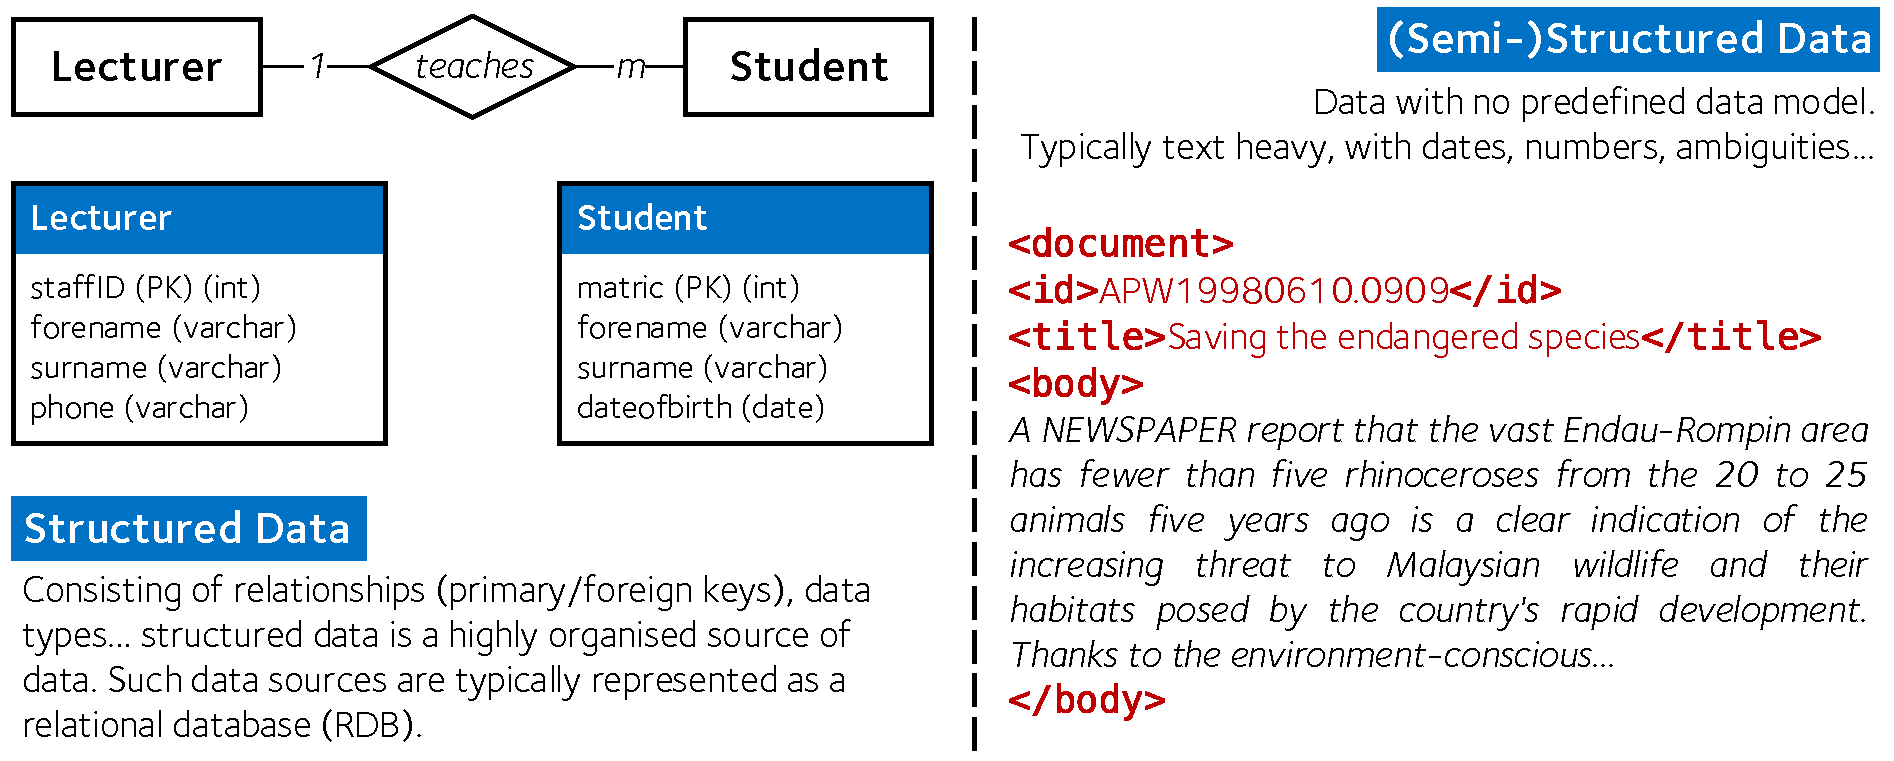
\includegraphics{figures/ch2-structured.pdf}}
    \caption[Structured and (semi-)structured data]{Examples of structured and (semi-)structured data. On the left is a structured~\gls{acr:rdbms} schema, represented in \emph{compressed Chen notation}~\citep{chen1976notation}. Different types can be specified for each field, representing data in a structured way. On the right, semi-structured data, using a document from a newswire collection. Note the semi-structured component at the top of the document (containing an identifier and title), and the unstructured body text.}
    \label{fig:structured_data}
\end{figure}

Being able to effectively sift through large volumes of unstructured data led to the development of retrieval systems. Consisting of a number of key components, the basic process of a retrieval system -- complete with \emph{searcher interactions} -- can be seen in Figure~\ref{fig:irs}. Core to the wider system is the \blueboxbold{retrieval engine}, of which many \emph{experimental}\footnote{\cite{rijsbergen1979ir} defines a difference between \emph{operational} and \emph{experimental}~\gls{acr:ir} systems. A majority of individuals will only ever interact with an operational system (such as Google). The work in this thesis however focuses more on experimental~\gls{acr:ir} systems, and the methodology employed to compare different experimental retrieval systems against each other.} systems can be selected based upon the requirements and existing infrastructure available. Examples include \emph{Lemur/Indri,} \emph{Lucene for~\gls{acr:ir}}, \emph{Okapi,} the \emph{Terrier~\gls{acr:ir} platform,} \emph{Wumpus} and \emph{Zettair.} Common to all systems are three key inputs, which are:

\begin{itemize}
    \item{an \blueboxbold{index} of documents, a specially crafted data structure used for the fast lookup of documents derived from a source collection, or \emph{corpus};}
    \item{a \blueboxbold{retrieval model} that scores and identifies documents that may constitute as relevant; and}
    \item{a \blueboxbold{query}, the construct that represents the searcher's \emph{information need.}}
\end{itemize}

\begin{figure}[t!]
    \centering
    \resizebox{1\hsize}{!}{
    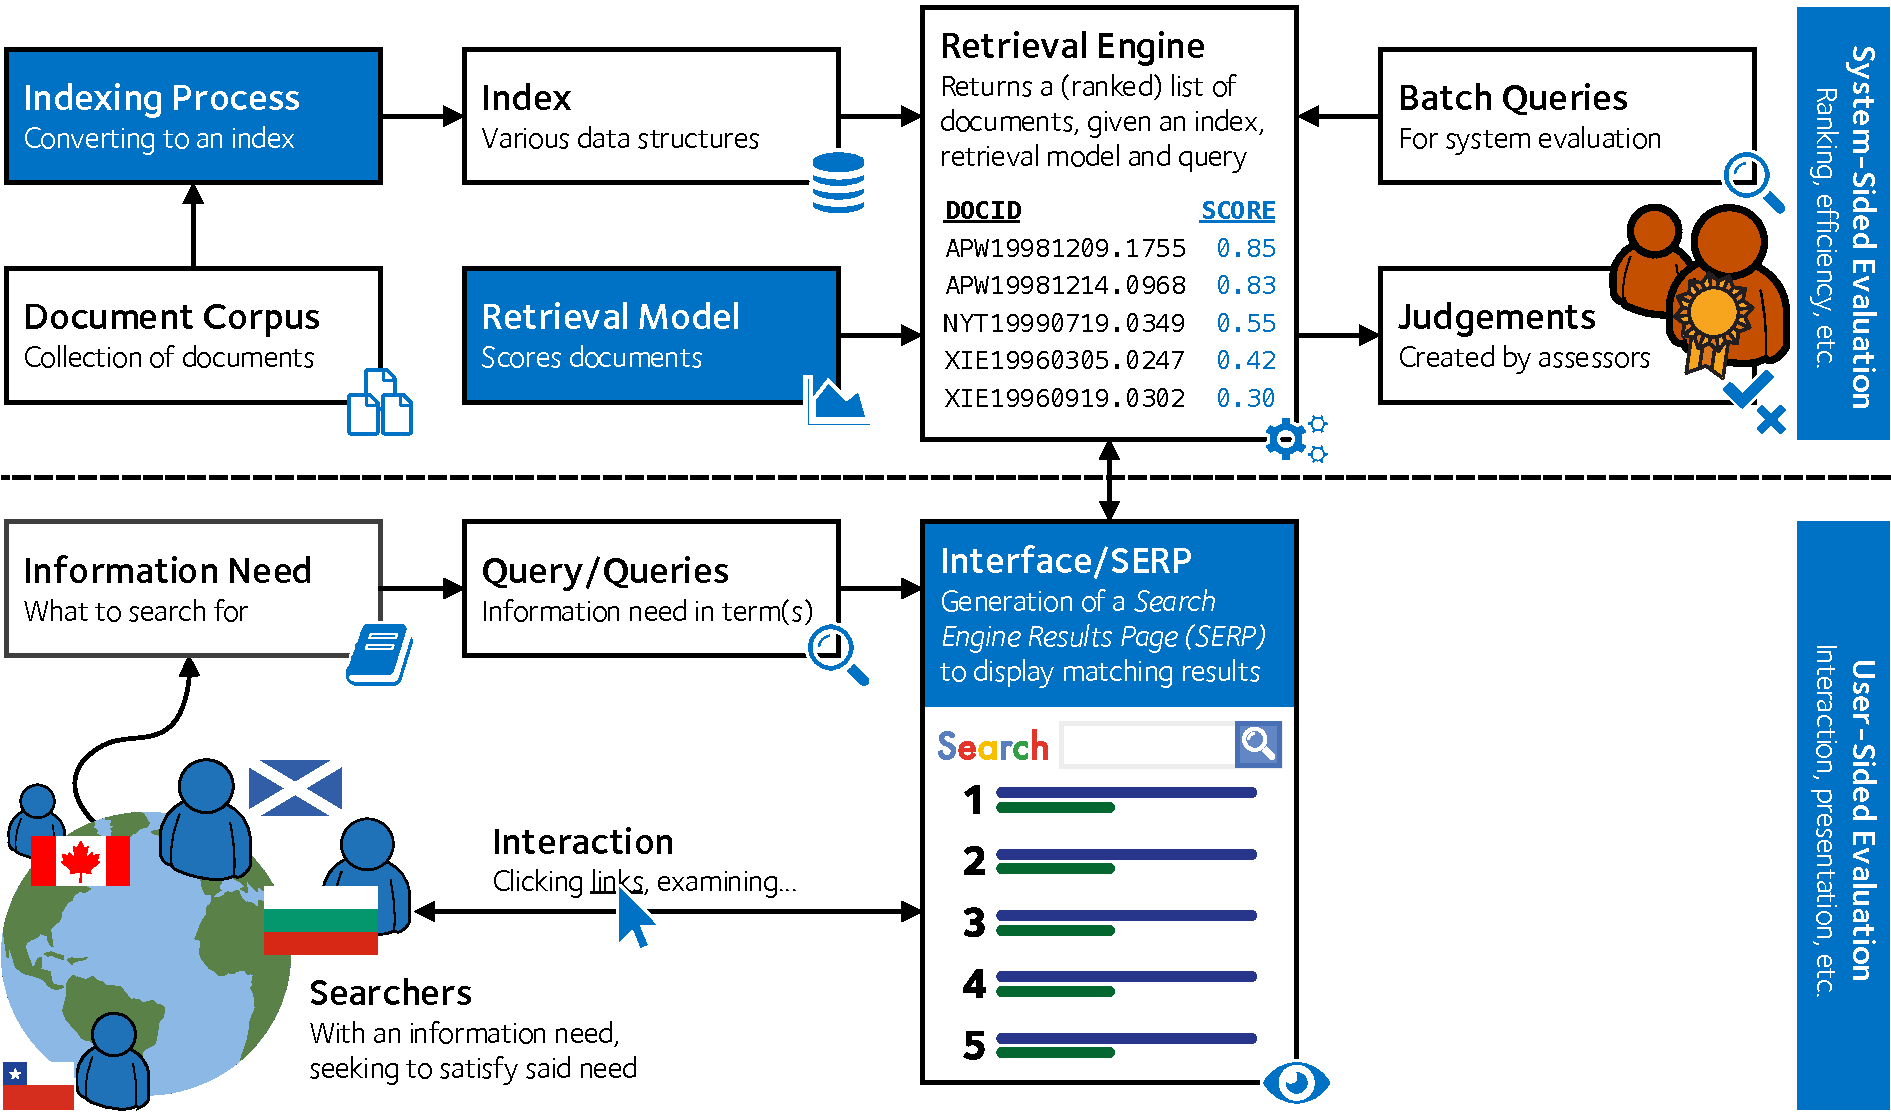
\includegraphics{figures/ch2-irs.pdf}}
    \caption[Basic components of a retrieval system]{The basic components of an~\gls{acr:ir} system, including the \emph{index, retrieval model} and a \emph{query.} Core to the entire process is the \emph{retrieval engine,} responsible for matching documents against said query. Also included in this diagram are nods to both \emph{system} and \emph{searcher} evaluation, discussed in depth later in this chapter.}
    \label{fig:irs}
\end{figure}

The retrieval engine combines these inputs to yield an output. This is typically a \emph{ranked} list of documents that the retrieval model believes to offer relevant documents to the issued query -- often called the \emph{matching process.} The query is formulated by the \blueboxbold{searcher} that is utilising the retrieval system; this stems from some information need that the searcher develops. Searchers then are \blueboxbold{presented} with results, formed as part of a~\glsfirst{acr:serp}, before they begin a series of different \blueboxbold{interactions} during a search session~\citep{ingwersen2005theturn}. These interactions provide the basis of the~\gls{acr:iir} process, which we discuss in \todo{\ref{sec:}}.

Additionally, the interactions that take place, or the system itself, can be evaluated to determine how \emph{efficient} or \emph{effective} the searcher or system is. System-sided evaluation will consider a series of ground truths, or \emph{relevance assessments,} to provide a means of determining how good the results returned by the retrieval system are. Output can be evaluated using these assessments in conjunction with some \emph{evaluation tool,} producing different measures.

We now provide a more in-depth discussion of the key components of indexing and basic retrieval models, before we move onto a discussion of the \emph{interactions} that take place between a retrieval system and its searchers.

\subsection{The Indexing Process}
The process of indexing takes into account the conversion of a collection of documents (or corpus) into a data structure that facilitates fast, full-text search -- a key requirement of any retrieval system. This full-text search is typically undertaken in milliseconds, with the goal of finding documents that will be relevant to a given query (and thus information need). The additional storage space and management requirements to maintain an index of documents is considered to be a necessary tradeoff to guarantee timely responses to searcher queries.

As illustrated in Figure~\ref{fig:inverted}, the indexing process can be split into three main steps:

\begin{itemize}
    \item{gathering the corpus of documents to be indexed;}
    \item{performing pre-indexing data preparation; and}
    \item{creating the index.}
\end{itemize}

Experimental corpora are available for use with batch experimentation, typically for \todo{various evaluation forums.} For operational retrieval systems, data is collated by other means. For example, web search engines employ a \emph{web crawler} to examine pages on the~\gls{acr:www}, and accumulates more content by following the~\glsplural{acr:www} hyperlink structure. Google's crawler, \emph{Googlebot,} regularly crawls high impact websites to ensure that the associated index is continually refreshed with up to date information.

\begin{figure}[t!]
    \centering
    \resizebox{1\hsize}{!}{
    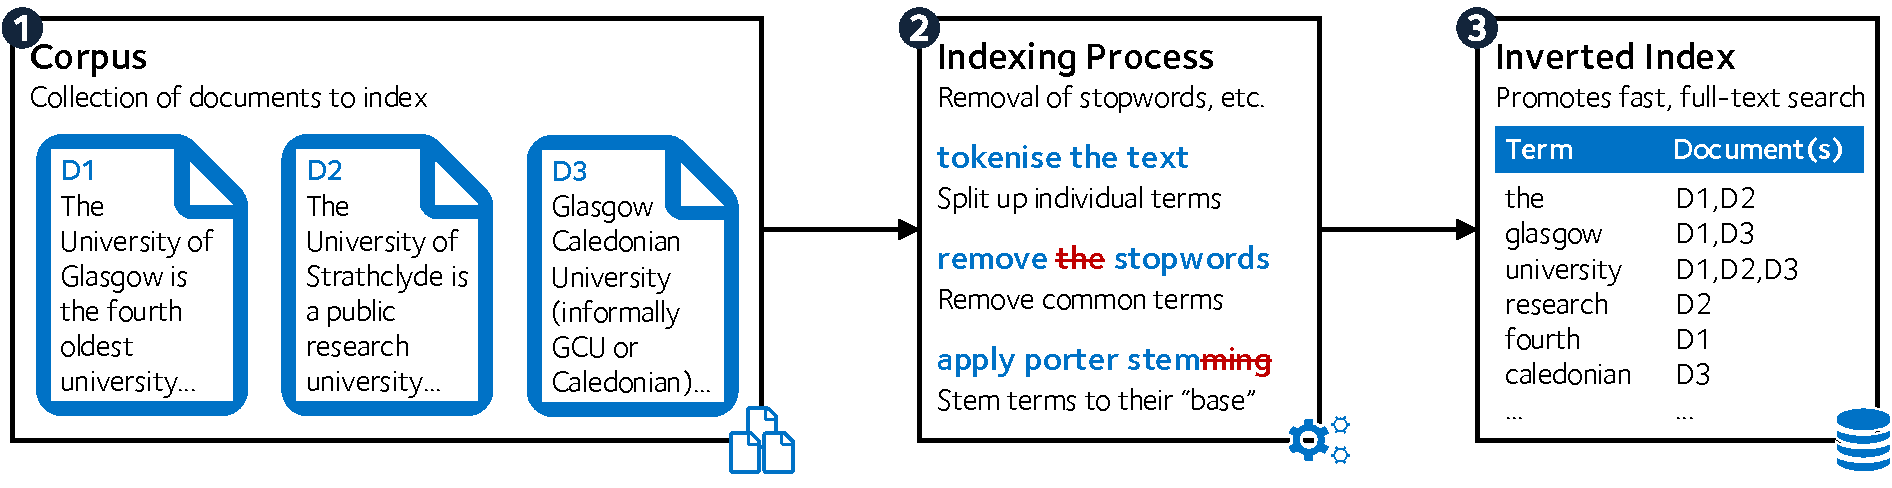
\includegraphics{figures/ch2-inverted.pdf}}
    \caption[Illustration of an \emph{inverted index}]{A demonstration of an \emph{inverted index}, with three source documents for comparison. Depending upon the requirements of the~\gls{acr:ir} system, the indexing process may vary; all classical~\gls{acr:ir} systems however rely upon some form of inverted index.}
    \label{fig:inverted}
\end{figure}

An index will contain an entry for each processed document, along with a \emph{vector of terms} that are present within said document. This is known as the \emph{forward index.} A retrieval system however needs to support fast full-text search, matching terms from a searcher's query to one or more documents within the index. To support faster query matching, the most simplistic approach is to simply \emph{invert} the index, such that the lookup of the index then corresponds to individual terms, not individual documents. A \emph{vector of documents} can then be provided for each term, yielding much faster access to a potential list of documents. An example of an inverted index is provided in Figure~\ref{fig:inverted}. The source corpus in this example illustration consists of three documents, and the resultant inverted index is shown. The set of documents retrieved can then be sent to a retrieval model for ranking.

Before a document is indexed however, a number of pre-indexing steps usually take place. Three of the most common processes involved within such a pipeline include \emph{tokenisation,} \emph{stopword removal} and \emph{stemming.}

\subsubsection{Tokenisation}
Put simply, tokenisation is the process of \emph{parsing} a source document, and splitting the data within the document into a number of individual \emph{tokens} that may be subsequently indexed. A token is considered a sequence of characters, grouped together to be semantically useful for processing its given document. While we do not go into greater deeper about the process of tokenisation, there are many challenges to this process -- such as \emph{word boundary ambiguity}. While parsing an English or Latin-based document may be relatively straightforward (with spaces representing \emph{word boundaries}), what about other languages, such as Chinese or Japanese? Considering what words a potential searcher of a retrieval system may use to search with may be a potential pathway for finding a solution to this problem.

\subsubsection{Stopword Removal}
Stopword removal is another popular choice for indexing document collections for an experimental~\gls{acr:ir} system. Illustrated in Figure~\ref{fig:inverted}, extremely common words which would appear to have little value in selecting documents matching a searcher's query (that is, \emph{non-discriminative} words) can simply be removed from a document's vocabulary entirely. Examples of such words could be \emph{the}, \emph{a}, or \emph{did}, or even a complete phrase from the famous soliloquy of William Shakespeare's \emph{Hamlet:} \emph{``to be or not to be''.} Such words are regarded as \emph{stopwords}. Some experiments consider a small list of stopwords, while others consider a larger list, with larger lists often significantly reducing the size of an indexed corpus~\citep{manning2008ir}. Indeed, it was argued by~\cite{fox1992stopwords} that larger lists ``are advisable''.

While stopword lists may be manually crafted under particular scenarios, automatic extraction from a document corpus is perhaps a more common practice. A simple approach would be to count the \emph{term frequency} for each term within a corpus, and sort the resultant list in descending order, selecting some top \emph{k} of the most frequently occurring terms. Readily available lists are also available.~\cite{rijsbergen1979ir} for example produced a list of 250 terms, with~\cite{francis1985stopwords} demonstrating a list of 425 stopwords from the \emph{Brown corpus}\footnote{The \emph{Brown corpus} was a collection of documents representing (then) contemporary American English, compiled by William Francis and Henry Ku\v{c}era -- refer to~\cite{francis1979brown_manual} for more information.}. For the experiments detailed in this thesis, \emph{Fox's classical stopword list}~\citep{fox1992stopwords} is used, consisting of 421 terms. Such an approach may be considered fine, but stopwords lists do vary from collection to collection, as stated by~\cite{lo2005automatically}.

Issues of course also exist with the removal of stopwords. Removing stopwords from a query may decrease processing time, but what if all terms within a query are stopwords? The resultant query passed to the retrieval engine could contain zero terms! As such, commercial retrieval systems are less likely to employ stopword removal to counter such an occurrence~\citep{manning2008ir, dolamic2010stopword}. Techniques such as compression may be employed to keep the size of the resultant index down. Queries such as \texttt{`to be or not to be'} may well contain some semantical meaning. Like tokenisation, there is often more to this problem than meets the eye.

\subsubsection{Stemming}
Another common pre-indexing process is \emph{stemming} (also called \emph{lemmatisation).} This is the process of reducing inflected -- or sometimes derived -- words from their \emph{word stem, base} or \emph{root.} For example, given the terms \texttt{fisher}, \texttt{fished} and \texttt{fishing}, reducing each of these terms to their respective word stem would result in \texttt{fish}. Essentially, stemming allows one to group words together with a similar, basic semantical meaning. This provides the advantage of reducing the size of an index, with fewer terms to index. A further benefit may be the potential increase in the number of possible matches that can be found with a stemmed set of query terms, increasing the retrieval system's \todo{\emph{recall.}}

The concept of stemming has been studied since the 1960's, with the \emph{Porter stemmer}~\citep{porter1980algorithm} emerging over time as empirically the most effective.\footnote{The Porter stemming algorithm is not provided in this thesis; refer to~\cite{porter1980algorithm} for an in-depth explanation of the algorithm.} Comprised of a series of linguistic rules, the \emph{measure} of a word can be considered, where \emph{``loosely checking the number of syllables to see whether a word is long enough that it is reasonable to regard the matching portion of a rule as a suffix rather than as part of the stem of the word.''}~\citep{manning2008ir}. Porter stemming is utilised in the indexing process for the work reported in this thesis; other stemmers do exist, with examples including the original single pass stemmer devised by~\cite{lovins1968development}, and the Krovetz stemmer~\citep{krovetz1993stemming}.

Issues such as \emph{overstemming} can impact upon the performance of a retrieval system. This is when terms are reduced back too far to the point that it loses meaning -- and can thus negatively affect the results returned. Terms like \texttt{universe}, \texttt{university} and \texttt{universal} when stemmed will be reduced to \texttt{univers}. While the three original terms may be etymologically linked, their modern meanings are however very different. If stemming is applied like so, documents containing both \texttt{universe} and \texttt{university} could be returned. While we do not go into depth into the solutions to this problem in this thesis, one potential solution is to consider the \emph{$n$-gram} context of a given term, allowing the retrieval system to thus select the correct step for the term~\citep{mcnamee2005stemminggrams}.

\subsection{Retrieval Models}
Given a generated document index and a searcher's query, the next part of the process is retrieval, or \emph{matching.} For this, a number of mathematically-based \emph{retrieval models} have over the years been developed that attempt to operationalise the notion of relevance. Such models provide us with a means for discussion and further refinement. They also provide us with the blueprint from which we operationalise a retrieval system~\citep{hiemstra2009ir_models}. The usefulness of such a model can be subsequently tested via experimentation and evaluation.

Several different types of retrieval model have been defined, ranging from the relatively simplistic, to the more complex. More complex approaches not only define a notion of what documents would be considered relevant, but also to what \emph{degree} that is so. This section considers four main retrieval model families, including:

\begin{itemize}
    \item{the \emph{boolean model;}}
    \item{the \emph{vector space model;}}
    \item{\emph{probabilistic models;} and}
    \item{more recent \emph{language models.}}
\end{itemize}

While not totally exhaustive -- approaches such as contemporary \emph{neural~\gls{acr:ir} models}~\citep{mitra2017neural_ir} are not considered here, for example -- this broad overview provides a solid understanding of the developments of such models, and the benefits and disadvantages of each approach. We focus the discussion of each retrieval model with an emphasis on how it can potentially influence the stopping behaviours of searchers.

\subsubsection{Boolean Model}
Cited as the first formally defined~\gls{acr:ir} retrieval model, the boolean model is also the most likely one to be criticised~\citep{hiemstra2009ir_models}. The model employs operators of mathematical logic as defined by George Boole~\citep{boole1847mathematical}, or \emph{set theory.} Boole defined three basic operators: \texttt{AND}, yielding a logical product between two sets; \texttt{OR}, yielding the logical sum between two sets; and \texttt{NOT}, yielding the logical difference.

\begin{figure}[t!]
    \centering
    \resizebox{1\hsize}{!}{
    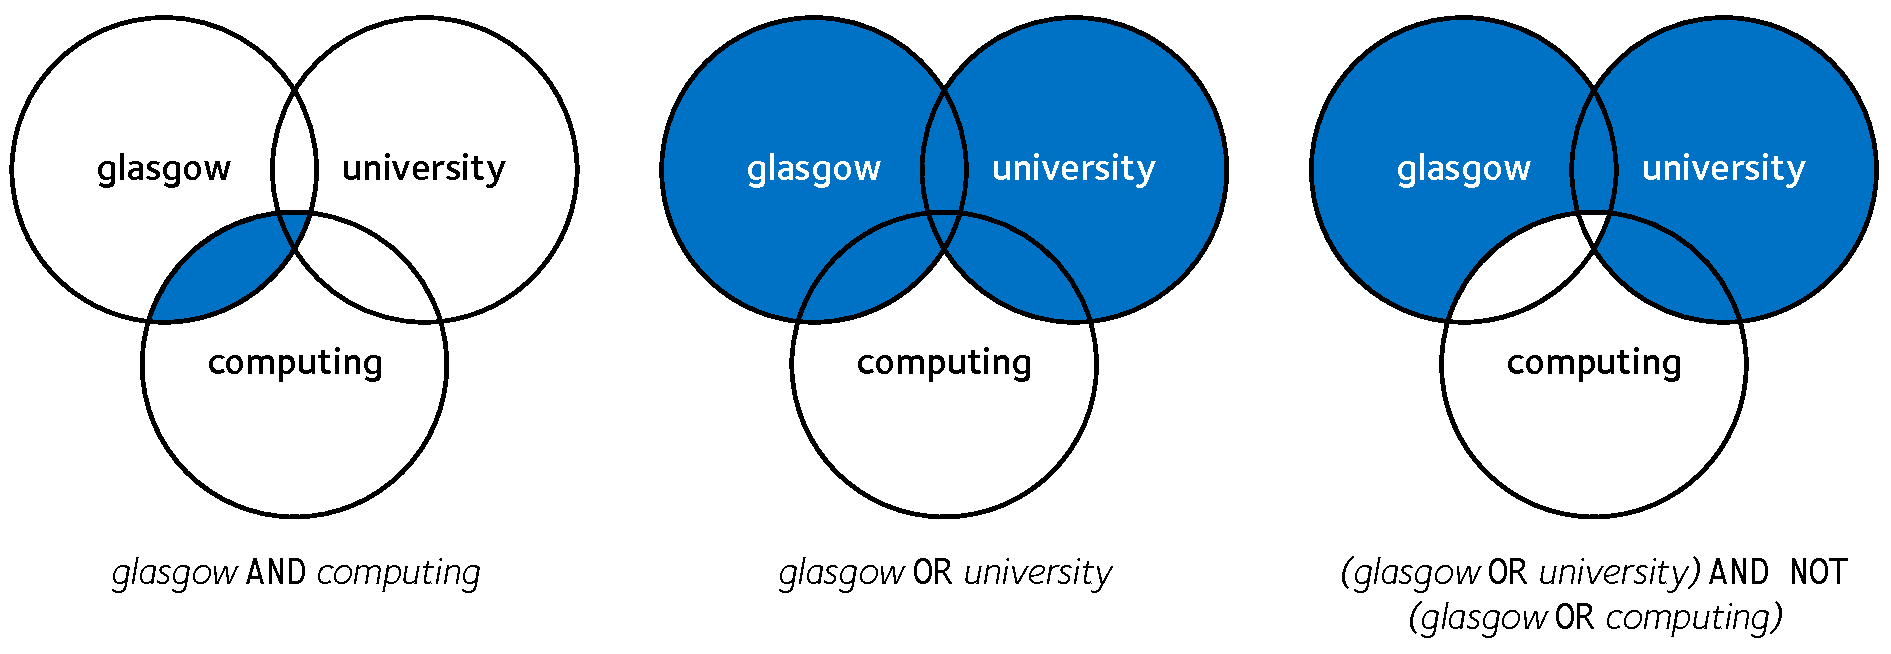
\includegraphics{figures/ch2-boolean.pdf}}
    \caption[Venn diagrams illustrating boolean retrieval]{An example illustration of the boolean retrieval model, using the query terms \texttt{glasgow}, \texttt{university} and \texttt{computing}. Each disc represents the set of documents containing that particular term. In the figure, three Venn diagram examples are provided, demonstrating the key logical operators used (\texttt{AND}, \texttt{OR} and \texttt{NOT}). Areas in blue are returned in the example boolean query provided underneath each Venn diagram.}
    \label{fig:boolean}
\end{figure}

By considering an individual query term and an unambiguous set of documents, logical operations can be applied to retrieve a set of documents. For example, the query term \texttt{glasgow} will yield a set of all documents containing the term \texttt{glasgow}, yet the query \texttt{NOT glasgow} will retrieve the set of documents that \emph{do not} contain any mention of the term \texttt{glasgow}. These results of applying logical operators between different sets can be illustrated through a \emph{Venn diagram,} where each set of documents is represented as a disc. Figure~\ref{fig:boolean} provides an example of such diagrams, using \texttt{glasgow university computing} as an example.

Despite its relative simplicity, there are major limitations to the exact match approach. First, when considering the boolean query, there is no notion of term importance -- every term has equal weighting. Querying utilising logic rules also appear as relatively unnatural representations of the searcher's information need. Indeed, as an information need becomes more complex, the corresponding boolean query can grow to be disproportionally large and cumbersome to interpret. As documents either belong to a set or not, a document is considered to be either relevant \texttt{(TRUE)} or not \texttt{(FALSE)}. As such, one cannot estimate a degree to how relevant a document would be to the searcher's query, and thus results are provided to the searcher in an unranked manner.

Returning an unranked set of documents would appear as an alien concept to searchers of contemporary retrieval systems -- one would assume that the document presented first would be the document considered to have the greatest relevance, as per the underlying retrieval model. This would make it difficult for a searcher to obtain some notion of how many results he or she should examine before stopping -- no ranking means all returned documents are of equal importance. 

\begin{figure}[h]
    \centering
    \vspace{4mm}
    \resizebox{1\hsize}{!}{
    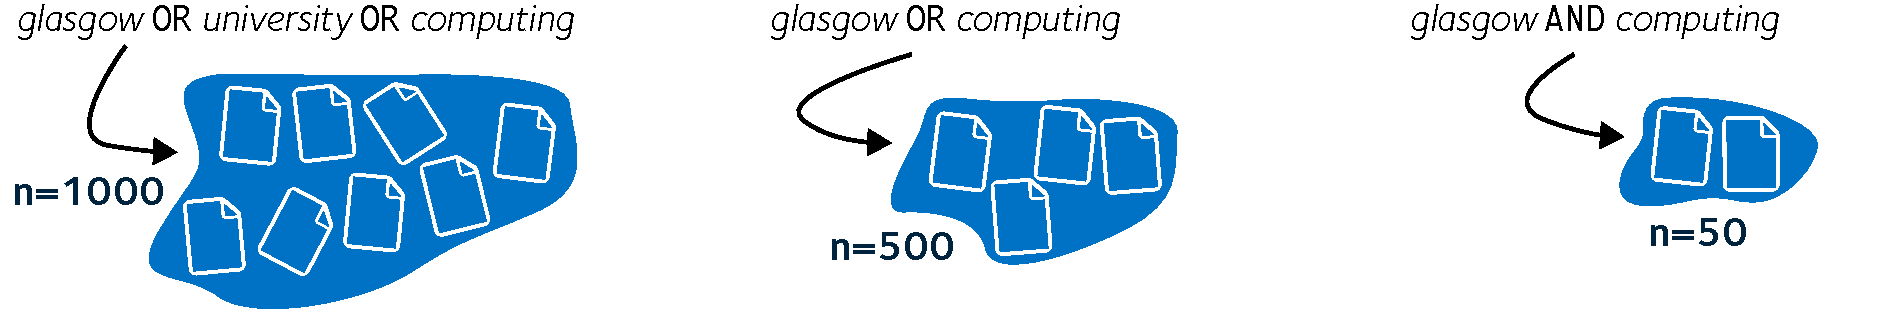
\includegraphics{figures/ch2-boolean-reduce.pdf}}
    \label{fig:searchbox}
    \vspace{-5mm}
\end{figure}

Instead, a searcher utilising a boolean retrieval system will often find an initial exploratory query will return a large set of documents, too many to examine each in sufficient detail. Rather, what a searcher will do is gradually reformulate their query -- like in the illustration above -- until the document set returned is of a manageable size, and small enough to process. This is an inherently different kind of stopping behaviour from the examples provided thus far in this thesis that assumes documents are presented in a \emph{ranked} list, with the notion of a stopping depth coming into play.

Despite not being required in contemporary retrieval systems, many systems still do provide support for crafting a boolean query for when returning a good set of results is difficult. Boolean queries may also be of use where ambiguity exists within a searcher's query, and clarification is required to eliminate a set of non-relevant documents. Indeed, boolean queries still find considerable traction in professional search systems, such as patent search. Here, missing an existing, relevant patent may be incredibly costly -- here, \emph{recall} is preferred over \emph{precision}, as discussed in \todo{Section~\ref{}.}

\subsubsection{Vector Space Model}
With major weaknesses present in the boolean retrieval model, work then progressed to develop more advanced approaches that mitigated the issued raised above.~\cite{luhn1957ranking_query} hypothesised that a searcher, when wishing to search for documents addressing their information need, should prepare a document that is similar to the documents being sought after. By comparing documents against this \emph{representative} document, a retrieval system could then begin to deduce what other documents would be useful, and by \emph{what margin.}

The vector space model proposed by~\cite{salton1975vsm} incorporates the principles as outlined by~\cite{luhn1957ranking_query}. These basic principles are operationalised by representing queries and documents within Euclidean geometry, where both are represented as vectors in multi-dimensional space. The notion of how close documents appear to each other denotes the relevance of a document.

The vector space model has been very popular, as it provides an intuitive means for addressing the overarching problem of a retrieval system. It can also incorporate methods such as \emph{term weighting,} which has been shown to improve retrieval effectiveness~\citep{croft2010search}. Furthermore, as queries and terms ad represented in Euclidean space, vector similarity methods can be employed to determine relevance. While many approaches have been trialled, empirical evidence have favoured \emph{cosine similarity}~\citep{croft2010search}. This is illustrated in Figure~\ref{fig:vector_space}. Using such an approach allows one to then compute the degrees of relevance, meaning that matched document can be returned in a ranked order. The ability of providing a ranking then permits searchers interacting with the results list to decide at what depth they should stop examining them. In other words, the ranking provides searchers with an \emph{estimate} as to when they should stop, or when the scores assigned to documents from a particular ranking begin to fall below an acceptable threshold.

\begin{wrapfigure}[13]{r}{0.45\textwidth}
    \begin{center}
    \vspace*{-10mm}
    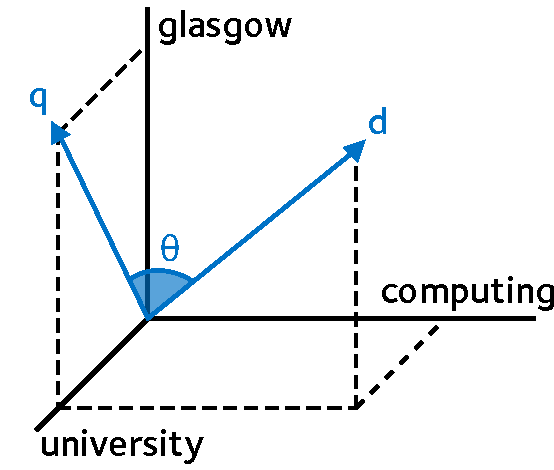
\includegraphics[width=1\textwidth]{figures/ch2-vector.pdf}
    \end{center}
    \vspace*{-4mm}
    \caption[Vector space model (cosine similarity)]{An illustration of the vector space model in Euclidean space, with each term representing a dimension. Here, the cosine similarity between query \emph{q} and document \emph{d} is shown.}
    \label{fig:vector_space}
\end{wrapfigure}

In order to understand the basic workings of the vector space approach, let us consider a query, $Q$, with each of its constituent terms placed within a term vector in $t$-dimensional space, leading to $Q = (q_1, q_2, q_3,\dotsc, q_{it})$. Consider also a document, $D_i$, with terms from the document again represented in $t$-dimensional space, yielding $D_i = (d_{i1}, d_{i2}, d_{i3},\dotsc, d_{it})$. From this notation, $d_{ij}$ represents the \emph{term frequency (TF)} of term $j$ appearing in document $i$. With each term represented as a separate dimension within Euclidean space, a weighting scheme can be subsequently applied to emphasise or understate more discriminative or less discriminative terms, respectively. By applying weighting schemes, the vector space model ranks documents which promotes terms that are more discriminative, thus improving the quality of the returned ranked list.

Term frequency is one of many different term weighting schemes that have been trialled over the years in~\gls{acr:ir} research. Perhaps one of the best and widely used schemes is \emph{inverse document frequency (IDF)}, proposed by~\cite{sparck1972statistical}. Here, the frequency of a term is normalised against the length of a given document. In the words of its creator, IDF allows for one to define the specificity of a term as \emph{``an inverse function of the number of documents in which it occurs.''}~\citep{sparck1972statistical}. This is useful as non-discriminative terms that occur frequently within an index (e.g. \texttt{the}) would have a small weighting applied, with the inverse happening for more discriminative terms, better able to describe a given document.

TF and IDF are typically combined together as a measure of both term appearance and importance, under an approach called \emph{TF-IDF}. For a given term $k$, one can calculate a TF-IDF score with the following equation:

\begin{equation*}
tf_{i,k} \cdot idf_{k} = \frac{f_{i,k}}{\sum_{j=1}^{t} f_{i,j}} \cdot log \frac{N}{n_k}.
\end{equation*}

Above, $f_{i,k}$ is the frequency of term $k$, $N$ is the number of documents in the collection used, and $n_k$ is the number of documents in which term $k$ appears at least once.


\subsubsection{Probabilistic Models}
The next major development were probabilistic retrieval models, defined to estimate the likelihood of a document being relevant to a given query. One of the most well known ranking principles, known as the \emph{Probability Ranking Principle (PRP)} -- defined by~\cite{robertson1977prp} -- who in turn attributed the development to~\cite{cooper1971relevance} -- states the following:

\begin{quote}
\emph{``If a reference retrieval system's response to each request is ranking of the documents in the collections in order of decreasing probability of usefulness to the user who submitted the request, where the probabilities are estimated as accurately as possible on the basis of whatever data has been made available to the system for this purpose, then the overall effectiveness of the system to its users will be the best that is obtainable on the basis of that data.''}
\attrib{\cite{robertson1977prp}}
\end{quote}

Essentially, this states that documents that are considered more likely to be relevant than non-relevant should be retrieved -- or where $P(R|D) < P(\overline{R}|D)$. However, while the PRP lays the much of the foundation from which probabilistic models have been derived, it does not provide its own concrete implementation of such a model.

Perhaps one of the most widely used derived models if \emph{Okapi BM25}~\citep{robertson1995trec3}. Indeed, this retrieval model has had considerable impact upon the~\gls{acr:ir} community, and is still used extensively today. BM25 provides a solid baseline for contemporary research, and is indeed the retrieval model employed in the experimentation discussed in this thesis, primarily for its effectiveness and popularity. Such a model, like the vector space model, again provides a ranking for documents returned -- and thus provides searchers with a gauge as to how relevant a document can be, given its ranking. Thus, it intrinsically provides a cue as to the depth at which a searcher should stop.

\subsubsection{Language Models}
The final retrieval model family that we discuss are language models, closely related to the probabilistic model we define above. Indeed, while such probabilistic models have been demonstrated to perform well empirically, adapting the PRP and subsequent developments to more advanced approaches has been difficult and is generally not intuitive~\citep{hiemstra2000language_modelling} -- the interpretation offered by probabilistic models may be considered loose, and is not always theoretically principled~\citep{whiting2015phd}. This has led to the development of more formalised statistical language modelling approaches, as defined in the fields of \emph{Natural Language Processing (NLP)}, for example~\citep{lavrenko2001language_models}.

Given the strong rooting in the principles of language and associated fields, language models provide a solution to the so-called \emph{bag of words}~\citep{harris1954distributional} concept that a majority of preceding retrieval models subscribe to. Put simply, this concept considers each document and query as a bag of words, meaning that the ordering of terms loses any significance. While a simplifying assumption, losing the ordering of terms means that semantic meaning and grammar rules are lost -- and thus a retrieval engine employing a model using this simplifying assumption may lose key meanings, and subsequently retrieval effectiveness will suffer.

Essentially, a language model is a probability distribution over strings of text. Given a string of text (i.e. a searcher's query), how likely is it that the given query appears in a given \emph{language}? Each document provides its own language, where we consider all possible phrases that the author of a document could have written when creating said document. Of course, some phrases are more likely than others. For example, the phrase \texttt{rain in glasgow} is more likely to appear in a document (in that order) than the seemingly random assortment of terms \texttt{purple monkey dishwasher}\footnote{If you ever watched \emph{The Simpsons}, you might disagree with this statement.}. Given this, and conceptualising a searcher's query in much the same fashion, we can produce a probability distribution $P(Q|D)$, concerning the probability of observing query $Q$ during some form of sampling within the language model of document $D$.

The most simplistic approach to language modelling is undoubtedly the \emph{unigram} approach, where each term within a document and/or query are considered in isolation, which subscribes to the aforementioned simplifying bag of words concept. Essentially, such an approach provides a probability distribution over the words appearing in the language. Higher order \emph{grams} such as \emph{bi-grams} and \emph{tri-grams} begin to consider more the place in which terms appear with respect to others, and thus the semantic meaning defined by this positioning begins to be taken into account within the probability distribution. When considering a document, the more a document discusses a particular topic, the more likely one would begin to observe terms about that topic in said document. When a term is not mentioned in a document, smoothing can be applied (given the wider collection the document is part of) to avoid a zero probability when calculating the probability of terms permitting the partial matching of queries where not all terms appear within a target document.


\section{From System to Searcher}
Considering the user -- what is IIR?
Core to their experience is the SERP as shown above.

Kelly has a spectrum of studies that consider the searcher.

From system-focused, to user focused.

Explain the IIR process.

\subsection{Presenting Results}
Core to the experience of a searcher is their interactions on a SERP. Explain the SERP, keep is simple and don't talk too much about the right rail.

\subsection{Cranfield and~\gls{acr:trec}}
- in the old history (rise of computers), there is a discussion about cranfield. bring it over here.
- explain TREC paradigm.

    Certain improvements have been made, time-biased gain.
        Like in TBG, look at snippet, some probability of document cost. snippet and document costs.
        simple markov model from vu's paper. This could go in the user models section.

\subsection{Searcher Models}

reiterate that there is a disconnect between the trec model (list assumptions), and reality.
and thus, people have worked on developing different models of the search process that better capture the IIR process.

2.3.1, bring it over, rephrased.
trec model of search.

start bringing over the stuff from chapter 3 in here.

\section{Evaluation Measures}

\subsection{System-Based Evaluation}

\subsubsection{Precision}

\subsubsection{Recall}

\subsubsection{Mean Average Precision}

\subsubsection{Expected Search Length}

\subsection{Searcher-Based Evaluation}

\subsubsection{Interactive Precision and Recall}

\subsubsection{Cumulative Gain Measures}

\subsubsection{Rank-Biased Precision}

\subsubsection{INST}

\section{Chapter Summary}